\chapter{Psalm 82}

\begin{figure}
  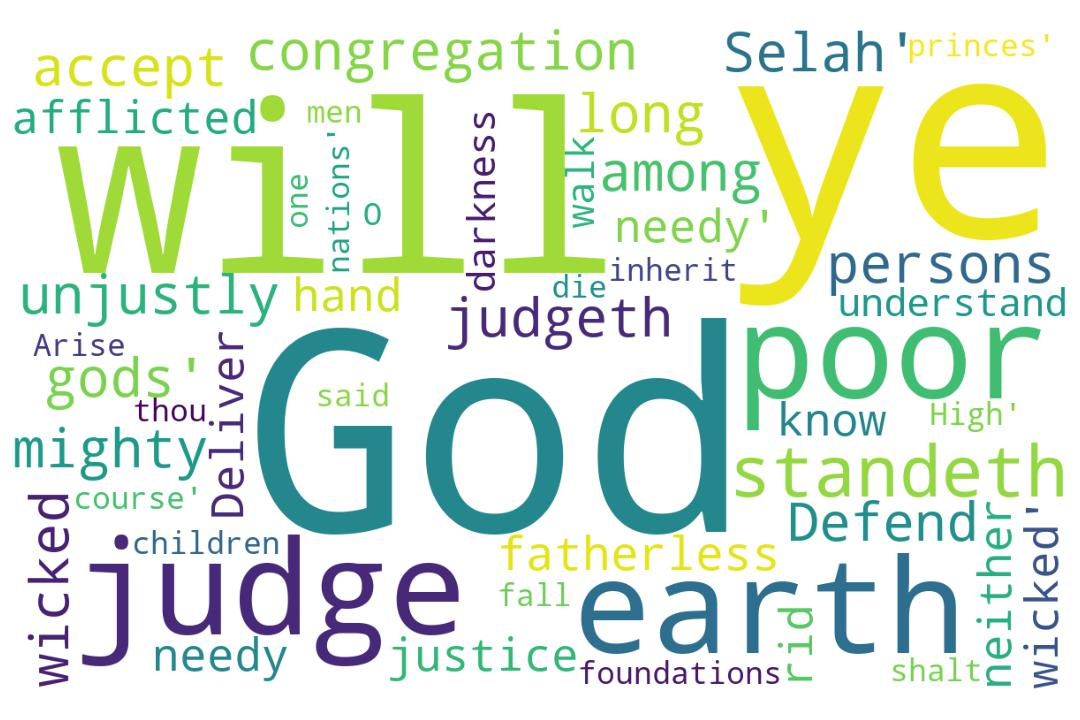
\includegraphics[width=\linewidth]{19OT-Psalms/Psalm82-WordCloud.jpg}
  \caption{Psalm 82 Word Cloud}
  \label{fig:Psalm 82 word Cloud}
\end{figure}

\marginpar{\scriptsize \centering \fcolorbox{bone}{lime}{\textbf{GOD IN CHARGE}}\\ (Psalm 81) \begin{compactenum}[I.][8]
   \item The \textbf{Realm of Leadership} \index[scripture]{Psalms!Psa 082:01}(Psa 82:1) 
    \item The \textbf{Ruin of a Leader} \index[scripture]{Psalms!Psa 082:02}(Psa 82:2) 
    \item The (Proper) \textbf{Regard of a Leader} \index[scripture]{Psalms!Psa 082:03}(Psa 82:3) 
    \item The \textbf{Rebuke of Leaders} \index[scripture]{Psalms!Psa 082:05}(Psa 82:5) 
    \item The \textbf{Reasons for Bad Leaders} \index[scripture]{Psalms!Psa 082:05}(Psa 82:5) 
    \item The \textbf{Return of THE LEADER} \index[scripture]{Psalms!Psa 082:08}(Psa 82:8) 
\end{compactenum}}

\marginpar{\scriptsize \centering \fcolorbox{bone}{yellow}{\textbf{COURT IN SESSION}}\\ (Psalm 81) \begin{compactenum}[I.][8]
   \item The \textbf{Delay} \index[scripture]{Psalms!Psa 082:02}(Psa 82:2) 
   \item The \textbf{Defense} \index[scripture]{Psalms!Psa 082:03}(Psa 82:3) 
   \item The \textbf{Deliverance} \index[scripture]{Psalms!Psa 082:04}(Psa 82:4) 
   \item The \textbf{Darkness} \index[scripture]{Psalms!Psa 082:05}(Psa 82:5) 
   \item The \textbf{Descent} \index[scripture]{Psalms!Psa 082:06}(Psa 82:6) 
   \item The \textbf{Death} \index[scripture]{Psalms!Psa 082:07}(Psa 82:7) 
   \item The \textbf{Disposing} \index[scripture]{Psalms!Psa 082:08}(Psa 82:8) 
\end{compactenum}}


\footnote{\textcolor[rgb]{0.00,0.25,0.00}{\hyperlink{PsalmsTOC}{Return to end of Table of Contents.}}}\footnote{\href{https://audiobible.com/bible/psalms_82.html}{\textcolor[cmyk]{0.99998,1,0,0}{Psalm 82 Audio}}}\textcolor[cmyk]{0.99998,1,0,0}{A Psalm of Asaph.}\\
\\
\textcolor[cmyk]{0.99998,1,0,0}{God standeth in the congregation of the mighty; he judgeth among the gods.}\footnote{\textbf{1 Kings 22:19} - And he said, Hear thou therefore the word of the LORD: I saw the LORD sitting on his throne, and all the host of heaven standing by him on his right hand and on his left.} %\footnote{But here, the spiritual truths give way to Biblical doctrines that are hard to hear, so those “dull of hearing” (Heb. 5:11) are now about to “bomb out” right and left. One will abort, one will miscarry, one will throw in the sponge, and another will move through the Psalm like a drugged sleep walker.\cite{Ruckman1992Psalms}}
[2] \textcolor[cmyk]{0.99998,1,0,0}{How long will ye judge unjustly, and accept the persons of the wicked? Selah.} %\footnote{“The congregation of the mighty” is not any congregation of earthly judges, and  when “he judgeth among the gods,” there is no reference to Israelite judges, any of Aaron’s seed, or anything else. Look at 1 Kings 22:19 for the Holy Spirit’s description of the “congregation of the mighty.” Verse 6 is what destroyed the spiritual sensibilities of Kroll, Duhm, Motyer, Clarke, Lange, Dummelow, Yates, Baethgen, Hengstenberg, and Charles Haddon Spurgeon. You will note that God often makes Charlie pay for his sin of leaning on the corrupt RV, at times, and occasionally aping Westcott and Hort by talking about “better renderings” and “better translations.” There is a price to pay for strutting like a peacock before the Holy Spirit. No man states the truth concerning the power and authority of the King James Bible any better than Spurgeon when he is in his right mind (see the Bible Believers’ Bulletin, September 1990), but alas, “all flesh is grass” and “all have sinned,” etc., so when Charlie tries to impress the stupid apostates of his day—who taught the faculties and staffs of every major Christian college and seminary everything they know—God puts him down as a candidate for blindness at a later date. This is one of those dates. That is the date line. It quickly eliminates every Nicolaitan who was trying to “bring out the intent of the original author” by “translating the Hebrew text in up to date language, so it might communicate to the receptor,” etc. (Interpretation: “He’s got a job that takes a lot of guts: he strings tennis rackets.”) \cite{Ruckman1992Psalms}}
[3] \textcolor[cmyk]{0.99998,1,0,0}{Defend the poor and fatherless: do justice to the afflicted and needy.}
[4] \textcolor[cmyk]{0.99998,1,0,0}{Deliver the poor and needy: rid \emph{them} out of the hand of the wicked.}
[5] \textcolor[cmyk]{0.99998,1,0,0}{They know not, neither will they understand; they walk on in darkness: all the foundations of the earth are out of course.}
[6] \textcolor[cmyk]{0.99998,1,0,0}{I have said, Ye \emph{are} gods; and all of you \emph{are} children of the most High.}
[7] \textcolor[cmyk]{0.99998,1,0,0}{But ye shall die like men, and fall like one of the princes.}\footnote{\textbf{Job 22:15-17} - Hast thou marked the old way which wicked men have trodden? 16 Which were cut down out of time, whose foundation was overflown with a flood: 17 Which said unto God, Depart from us: and what can the Almighty do for them?}\footnote{\textbf{2 Peter 2:4-5} - For if God spared not the angels that sinned, but cast them down to hell, and delivered them into chains of darkness, to be reserved unto judgment; 5 And spared not the old world, but saved Noah the eighth person, a preacher of righteousness, bringing in the flood upon the world of the ungodly;}% \footnote{You do not say: “I have said ye are cats, but ye shall die like cats.” You could say: “I have said ye are dogs, but ye will drown like fishes.” Two things that aren’t the same cannot be equated, so the scholars will have to “fix up” the “men” so they don’t stand in opposition to the “gods.” (That is what Scofield did with Genesis 6:2, so the “daughters of men” could simply be messing around with the “sons of men.” The text said “sons of God.”) This is fourth-grade English. The disjunctive conjunction (“but” vs. 7) shows us that we are not dealing with men; there are no human judges in verses 6–7. The contrast is between someone who might truly be a “god” but he will die like a man—not a “god.” Jamieson, Fausset, and Brown go to bat for every Biblecorrecting Nicolaitan at Liberty University and say that what the Holy Spirit meant to say in verse 7 was “not like any ordinary man.” This solves the problem for the Biblerejecting Fundamentalist who has no grasp of the Scriptures. “I have said you are above ordinary men, but you will die like ordinary men “; i.e., “I will tell you what the Scriptures should have said because as they are written it is impossible for me to understand them.” You see where this type of reasoning winds up? It winds up with “YOU need a different translation because the Holy Bible is impossible for YOU to understand. After all, if I, with my twenty five years of formal education, can’t understand it, how could YOU possibly understand it? Here! Buy this Nutty Imbecile’s Version (NIV). Cash, check, or money order!” See how it’s done? The judges in Genesis 6 corrupted the entire earth with their decisions. They made decisions worse than the ones made by the “nine old men” since 1933. These supernatural “gods” are identified as “gods” in the following places: Genesis 3:5; Exodus 15:11; Psalm 86:8, 95:3, 136:2 (Note THAT one! lmgine thinking those “gods” are Israelite judges!), and Jeremiah 10:11. They are called “the sons of God” in Job 38:7 and Genesis 6:2, so the only way Scofield could remove “children of the most High” from Psalm 82:6 was to pretend that the “gods” were NOT literally “the sons of God.” They were the “sons of Seth”! Had enough of “higher scholarship”? Is this enough from the “recognized scholars” whose “loyalty” to lost pieces of paper is “unquestioned”? Gotta belly full yet, or are you like the little boy who was told “If you eat one more bite, you are going to bust wide open”? He replied, “Please pass the cake and everybody stand back. “ The “gods” have been here before and will be here again. Idols are the mementos that man has used since the flood to commemorate their presence (see Isa. 44:10; Ps. 96:5, 97:7). They came down “in the likeness of men” according to the New Testament (Acts 14:11), so every angel in the Bible appears as a young man (Judg. 13:6; Gen. 19:5; Acts 1:10; Luke 24:4, etc.). Scofield got rid of them again by saying “angels are sexless.” But when he says “ye shall die like men,” he meant they would drown in the flood (2 Pet. 2:4–5; Job 22:15– 17), and so they did. At the time they were judging, Enoch was prophesying the Second Coming of Jesus Christ (see Jude 14). There is a chance that this Psalm may be a pre Deluge Psalm written by Enoch (see remarks under Ps. 90). All the commentators “blew it.” It is evident that once a man begins to mess with the King James text that the Author of Scripture begins to mess with his mind, and pretty soon he cannot get the simplest doctrinal and prophetic truths in order. This statement is proved the moment some blockhead on the faculty at Bob Jones, PCC, Santa Rosa, BBC, or Tennessee Temple tries to cover up his infidelity. We will cite an A 1 example, honed to perfection at Liberty University. Having been told that “all the foundations of the earth are out of course” (vs. 5)—which matches Isaiah 24:19–20—Kroll, of Liberty University, alters them to “the fabric of the nation.” (So help me, Delitzsch and Keil, that is what Lynchburg did with “the Hebrew text.”) ``Yet in the highly poetic language of the Psalm...when the fundamental basis of society, the very principles of morality, are not followed by the judges, the very fabric of the nation is shaken.'' Go sit on a tack. That is modern, “militant Fundamentalist” scholarship in 1992. It is a combination of stupidity, unbelief, arrogance, blindness, and equivocation wrapped up in one neat ball of piety and propagated by men who “don’t like Brother Ruckman’s language.” (I hope to God they don’t, and I hope to God they never will.) \cite{Ruckman1992Psalms}}
[8] \textcolor[cmyk]{0.99998,1,0,0}{Arise, O God, judge the earth: for thou shalt inherit all nations.} %\footnote{There it goes again, in case you missed the “Selah.” But at Liberty University they can’t find EITHER expression in ANY version. Kroll (absolutely spaced out) says that “Arise, O God” is just a “metaphor taken from the common gesture of judges who sit as they hear a case and rise up to pronounce a sentence.” No, that is exactly what the expression didn’t mean one time anywhere in the entire Bible. See Psalm 3:7, 7:6, 9:19, 10:12, 12:5, 17:13, 44:23, 26, 68:1, and 74:22. It wasn’t a “metaphor” one time out of ten. Trust Lynchburg to steal your money as well as your Bible. “For thou shalt inherit all nations” gave you the third clue as to the time, and Kroll still missed it. He had to apply the second half of verse 8 to the Second Advent because he was Premillennial, but being carnal (as well as stupid), he had to limit the first half of the verse to human judges before the Church Age. He, as everyone of his peers, ignored the fact that the ``gods'' will be here in the Tribulation, and they will be reigning not only as kings but as absolute authorities over all judicial matters on earth (Rev. 17:12). They will be in the same position as in Genesis 6:1--6. (Note the word “mighty,” as in Ps. 82:1.) When Christ applied the verse to human judges to prove His own deity (John 10:34--36), He knocked every translator, every reviser, every commentator, and every ``exegete'' slap out of the rink. At no time did God ever say “all of you Israelite judges are children of the most High.” To tell the truth, none of them were; not even the saved ones. The judges in Israel were Levites (Mal. 2:4, 7–8; Deut. 1:16, 21:5), and not one of them was a “child of God.” When John uses the expression (John 11:52), he uses it in a Jewish sense that was not doctrinal. Jesus Christ Himself allows that the Jews of that time were not only NOT the “children of God” (John 8:42--44), they were not even the children of Abraham (John 8:39). That isn’t all: “all the foundations of the earth” (vs. 5) were NOT “out of course” at anytime between Asaph and Paul, and they are not now, nor were they when Moses appointed human judges over Israel (Exodus 18:22, 25; Num. 11:16--17). Someone is “off their trolley” again; they have “one oar in the water.” The problem came from Exodus 22:28. With this and John 10:34, the Bible-correcting apostates took the liberty to throw out the entire context of Psalm 82, since they couldn’t understand it. The context (vss. 1, 5–6, 8) was the Second Advent, and the type was “the days of Noah,” for there the “gods” drowned like “men” (see vs. 7), at least according to 2 Peter 3:6; Jude 6; Job 22:16;  and Revelation 20:13 in the English text. There is nothing like Elizabethan English to make a debacle out of a seminary; especially if it is a bunch of book mad stuffed shirts who think the sun rises and sets on ``plenary, verbally inspired, original autographs.'' (A duck is a bird that walks like he has been riding a horse all day.) Dual application: The judges in Israel could be ``gods'' in the sense that Moses was a “god” to Pharaoh and Aaron (Exod. 7:1). You can be a ``son'' of God because you represent THE Son of God. (The Pope is not shy in the least; he simply applies God’s titles to himself, John 17:11.) The human judges could judge ``the poor and fatherless...the afflicted and needy...the poor and needy,'' so they acted as gods for these people. Final Authority. Get it? You got it yet? Christ merely quotes the passage to show that they have no right to accuse Him of claiming to be something that He is not. He doesn’t tell you one thing about the Psalm or what the Psalm was dealing with. So the Nicolaitans—who have been correcting the Psalms now for ten to three hundred years—can’t find out what is going on. When Christ says that it is written in the Law ``I said, ye are gods,'' the ``ye'' doesn’t have anything to do with anyone to whom He is talking who got ``the word of God.'' The ``ye'' was a reference to angels from Genesis 6 who will show up in the Tribulation. \cite{Ruckman1992Psalms}}

